\documentclass[12pt]{article}
\usepackage[english]{babel}
\usepackage{natbib}
\usepackage{url}
\usepackage[utf8x]{inputenc}
\usepackage{amsmath}
\usepackage{graphicx}
\usepackage{subcaption}
\graphicspath{{images/}}
\usepackage{parskip}
\usepackage{fancyhdr}
\usepackage{vmargin}
\usepackage[shortlabels]{enumitem}


\setmarginsrb{3 cm}{2.5 cm}{3 cm}{2.5 cm}{1 cm}{1.5 cm}{1 cm}{1.5 cm}

\title{MRI Quality Assurance}					% Title
\author{U.G.C. Jayasankha}								% Author
\date{\today}											% Date
\def \topic{MRI}

\makeatletter
\let\thetitle\@title
\let\theauthor\@author
\let\thedate\@date
\makeatother

\pagestyle{fancy}
\fancyhf{}
\rhead{\theauthor}
\lhead{\thetitle}
%\chead{170259P}
\cfoot{\thepage}

\begin{document}

%%%%%%%%%%%%%%%%%%%%%%%%%%%%%%%%%%%%%%%%%%%%%%%%%%%%%%%%%%%%%%%%%%%%%%%%%%%%%%%%%%%%%%%%%

\begin{titlepage}
	\centering
    \vspace*{0.5 cm}
    
\includegraphics[scale = 0.8]{University_of_Moratuwa_logo.png}\\[1.0 cm]	% University Logo
    \textsc{\Large Department of Electronics and Telecommunication Engineering}\\[0.8 cm]
    %\textsc{\Large University of Moratuwa}\\[1.0 cm]	% University Name
	\textsc{\large BM 3121}\\[0.5 cm]				% Course Code
	\textsc{\Large Medical Imaging}\\[0.5 cm]				% Course Name
	\rule{\linewidth}{0.2 mm} \\[0.4 cm]
	{ \huge \bfseries \thetitle}\\
	\rule{\linewidth}{0.2 mm} \\[1.5 cm]
	
	\begin{minipage}{0.4\textwidth}
		\begin{flushleft} \large
			\emph{Name:}\\
			\theauthor
			\end{flushleft}
			\end{minipage}~
			\begin{minipage}{0.4\textwidth}
			\begin{flushright} \large
			\emph{Index Number:} \\
			170259P									% Your Student Number
		\end{flushright}
	\end{minipage}\\[2 cm]
	
	{\large \thedate}\\[2 cm]
 
	\vfill
	
\end{titlepage}

%%%%%%%%%%%%%%%%%%%%%%%%%%%%%%%%%%%%%%%%%%%%%%%%%%%%%%%%%%%%%%%%%%%%%%%%%%%%%%%%%%%%%%%%%

\tableofcontents
\pagebreak

%%%%%%%%%%%%%%%%%%%%%%%%%%%%%%%%%%%%%%%%%%%%%%%%%%%%%%%%%%%%%%%%%%%%%%%%%%%%%%%%%%%%%%%%%

\section{Introduction to \topic}
\subsection{Basics of \topic}
Magnetic Resonance Imaging is a non-ionizing imaging modality which is capable of three dimensional scanning at a higher resolution compared with Computed tomography. MRI signal is generated from the protons in water and lipid molecules in the body. Protons in powerful magnetic field resonates when an electromagnetic wave is introduced. This behaviour is used for MRI. Since MRI uses superconductors at 0K, the cost of MRI is too high and maintenance is a big responsibility. MRIs take more time than X-ray imaging. Thus the patient should be hold stationary throughout the scanning. 

\begin{figure}[h!]
  \centering
  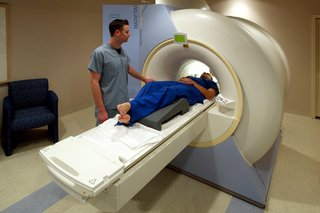
\includegraphics[width=0.5\linewidth]{mri.jpg}
  \caption{\small{MRI machine}}
  \label{fig:MRI machine}
\end{figure}

MRI technology was introduced in 1971. At the beginning it was known as Nuclear Magnetic Resonance Imaging (NMRI). But people were afraid to do imaging using this technology due to the misconceptions they had on the word nuclear. Then the "N" for nuclear was lopped off. So far MRI technology has developed a lot. In the beginning permanent magnets were used. Due to lack of magnetic field they were replaced by electromagnets.But due to their high power consumption superconductors were introduced to the MRI technology. To maintain superconductivity it is necessary to keep the temperature close to 0\textit{K}. Therefore the cooling system runs nonstop. When comparing with other imaging modalities this consumes more power but not more than the MRI which used non-superconductor electromagnets. 

MRI is used in wide range of body scanning such as brain, cranium, heart, liver, pancreas, lungs, kidneys, abdomen and pelvic cavity. MRI is used in several imaging methods such as Neuroimaging, Cardiovascular imaging, Oncology, Functional MRI, Musculoskeletal imaging and Gastrointestinal Imaging. 


\begin{figure}[h!]
  \centering
  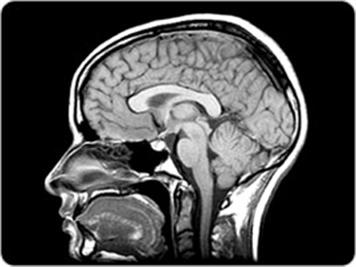
\includegraphics[width=0.45\linewidth]{MRI1.jpg}
  \caption{\small{MRI image of the head - Saggital plane}}
  \label{fig:MRI image of the head}
\end{figure}

\subsection{Importance of \topic}
MRI is a popular imaging modality due to following reasons.  
\begin{enumerate}
    \item Ionizing radiation is not used\newline
    X-ray, CT, PET modalities of imaging use ionizing radiation which is harmful for the organs. But in MRI ionizing radiation is not used. Therefore it is not harmful for the organs. 
    % \newline
    \item High soft tissue contrast \newline
    Most of other imaging modalities do not possess this much soft tissue contrast. But due to different relaxation times of the different kind of soft tissues MRI can detect, and contrast between different soft tissues.  
    
    \item High spatial resolution\newline
    In MRI spatial resolution can be around 1mm. By decreasing the the width of the slices, spatial resolution can be improved even more. But time used for the test gets increased. 
  
   % \newline
    \item Images can be 2D or 3D\newline
    3D image can be taken on any part of the body from the MRI machine, but the slices(2D) has much high resolution. 
    
    \item Negligible penetration effects\newline
    CT or X-ray uses a radiation source and passes the radiation through the body. But in MRI the relaxation generates EM radiation originated from the protons. Therefore the penetration effects are negligible. 
    
    \item Contrasts agents used are not harmful for the body\newline
    Contrast agents used in X-ray or CT affects the body. But the the contrast agents used in MRI do not have such effect.
\end{enumerate}
But there are several disadvantages also. 
\begin{enumerate}
    \item MRI systems are very expensive. Maintenance is a big responsibility.  
    \item People with metal implants can not use MRI for imaging.
    \item MRI scans take a longer time for the image acquisition. Patients have to stay in the MRI machine for 30-40 minutes. People with Claustrophobia can not resist such a situation. 
    \item MRI systems are extremely complex and any small fault would cost millions of rupees. 
\end{enumerate}


\subsection{Components and Implementation of \topic}
\begin{figure}[h!]
    \centering
    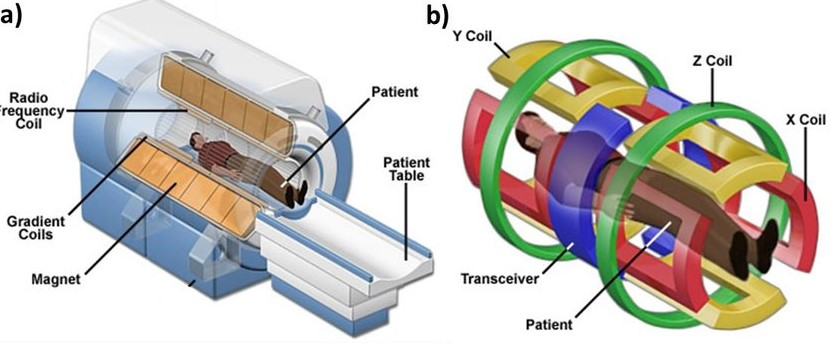
\includegraphics[width=\linewidth]{sys.png}
    \caption{\small{Main components of MRI system}}
    \label{fig:Main components of MRI system}
\end{figure}

Patient is entered through a hole in the machine. Around the patient there are several layers of different components. 

Components of the \topic ,
\begin{enumerate}
    \item Powerful superconductor magnet - 1.5T / 3T / 6T
    \item Gradient coils
    \item Radio Frequency coils
    \item Patient table
    \item Shield
    \item Computer system
    
\end{enumerate}

\pagebreak
\section{Quality Assurance of \topic}

The quality of the MRI system is very important in providing a better health service. The medical diagnosis based on magnetic resonance imaging depends on the fact that the image is sufficiently suitable to extract required information. Therefore quality assurance must be guaranteed. Otherwise diagnosis will be failed. The MRI system consists of many units as mentioned in above topic. Quality assurance of each part or section assures the quality of overall system. 

Furthermore, due to powerful magnetic properties, it is necessary to implement rules and regulation when implementing a MRI system and when using the MRI system. As an example; no one can enter the MRI room with any metallic equipment. If those rules are not implemented, there can be severe damages to the people in the room even death. Furthermore there can be damages to the system which definitely cost lots of money to recover. Therefore to assure the quality those rules and regulations are important. 

To assess the quality of MRI systems under the discussed aspects several parameters have been defined and agreed upon by the medical community internationally, regionally or institutionally. Regular tests should be done daily, weekly, monthly, quarterly or annually according to the requirement to identify and correct problems with MRI systems. 

The quality assurance of MRI is responsibility of following people - Quality Assurance Committee. 
\begin{enumerate}
    \item Radiologists
    \item MRI Technologists
    \item Medical Physicists/MRI Scientists
\end{enumerate}
This team should ensure that,

\begin{enumerate}[i.]
    \item Every imaging procedure is necessary and appropriate to the clinical problem at hand
    \item The images generated contain information critical to the solution of the problem
    \item The recorded information is correctly interpreted and made available in a timely fashion to the patient’s physician
    \item The examination results in the lowest possible risk, cost, and inconvenience to the patient consistent with objectives above
\end{enumerate}
\subsection{Radiologists' main responsibilities}
\begin{enumerate}[i.]
    \item Ensure that technologists have adequate training and continuing
education in MRI.
    \item Provide an orientation program for technologists based on a
carefully established procedures manual (see Section E).
    \item Ensure that an effective QC program exists for all MR imaging
performed at the site. The supervising radiologist should
provide motivation, oversight, and direction to all aspects of
the QC program.
    \item Select the technologist to be the primary QC technologist,
performing the prescribed QC tests.
    \item Ensure that appropriate test equipment and materials are available
to perform the technologist’s QC tests.
    \item Arrange staffing and scheduling so that adequate time is available
to carry out the QC tests and to record and interpret the results.
    \item Provide frequent and consistent positive and negative feedback
to technologists about clinical image quality and QC procedures.
    \item Participate in the selection of a qualified medical physicist or
MRI scientist who will administer the QC program and perform
the physicist’s tests.
    \item Review the technologist’s test results at least every three months,
or more frequently if consistency has not yet been achieved.
    \item Review the results of the qualified medical physicist or MRI
scientist annually, or more frequently when needed.
    \item Oversee or designate a qualified individual to oversee the MRI
safety program for employees, patients, and other individuals in
the surrounding area.
    \item Ensure that records concerning employee qualifications, MRI
protocols, and procedures, QC, safety, and protection are
properly maintained and updated in the MRI QA Procedures
Manual
\end{enumerate}

\pagebreak 
\subsection{MRI technologists' main responsibilities}
The MRI QC technologist’s responsibilities revolve around image quality. More specifically, the functions performed by the technologist that affect image quality are patient positioning, image production, image archiving, and film processing.

Following figure shows the quality assurance methods followed by MRI technologists and the frequency they are executed. 
\begin{figure}[h!]
    \centering
    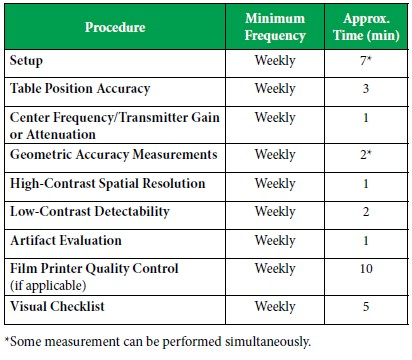
\includegraphics[width=0.8\linewidth]{testlist.jpg}
    \caption{\small{Minimum Frequencies of Performing Technologist’s QC Tests}}
    \label{fig:Minimum Frequencies of Performing Technologist’s QC Tests}
\end{figure}
\subsection{Medical Physicists/MRI Scientists' main responsibilities}
The responsibilities of the qualified medical physicist or MRI scientist relate to equipment performance, including image quality and patient safety.

Following figure shows the the quality assurance methods to be followed by MRI scientists.  
\begin{figure}[h!]
    \centering
    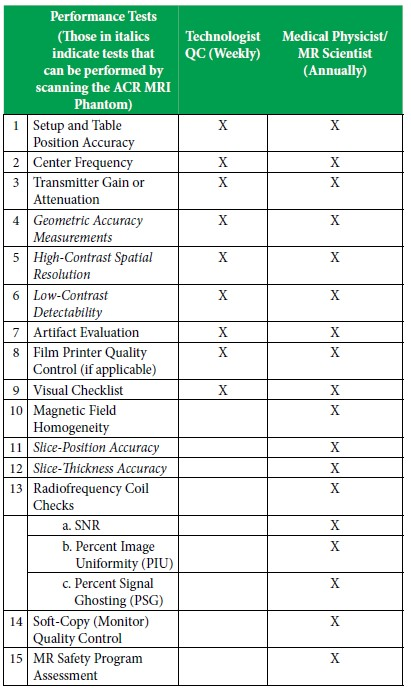
\includegraphics[width=0.75\linewidth]{ls.jpg}
    \caption{\small{Specific Required Tests Required for Annual MRI System}}
    \label{fig:Specific Required Tests Required for Annual MRI System}
\end{figure}
\pagebreak
\section{Main Quality Assurance Methods of MRI}
\subsection{Visual Checklist}
This is the basic method to find flaws in the system and it should be done in every week. Following list of equipment is inspected visually to find any missing part or any malfunction. This verifies whether the MRI system working properly electrically and mechanically. 

\begin{enumerate}
    \item Patient Transport and Gantry
    \begin{enumerate}
        \item Table position and other displays
        \item Alignment lights
        \item Horizontal smoothness of motion and stability
        \item Vertical motion smoothness and stability
    \end{enumerate}
    \item Filming Viewing
    \begin{enumerate}
        \item Laser camera
        \item Light boxes
    \end{enumerate}
    \item RF Integrity and Control Room
    \begin{enumerate}
        \item RF door contacts
        \item RF window-screen integrity
        \item Operator console switches/lights/meters
        \item Patient monitor and intercom
        \item Room temperature and humidity
    \end{enumerate}
    \item Facility Safety
    \begin{enumerate}
        \item Emergency cart
        \item Safety warning signage
        \item Door indicator switch
        \item Cryogen level indicator
    \end{enumerate}
\end{enumerate}
\begin{figure}[h!]
    \centering
    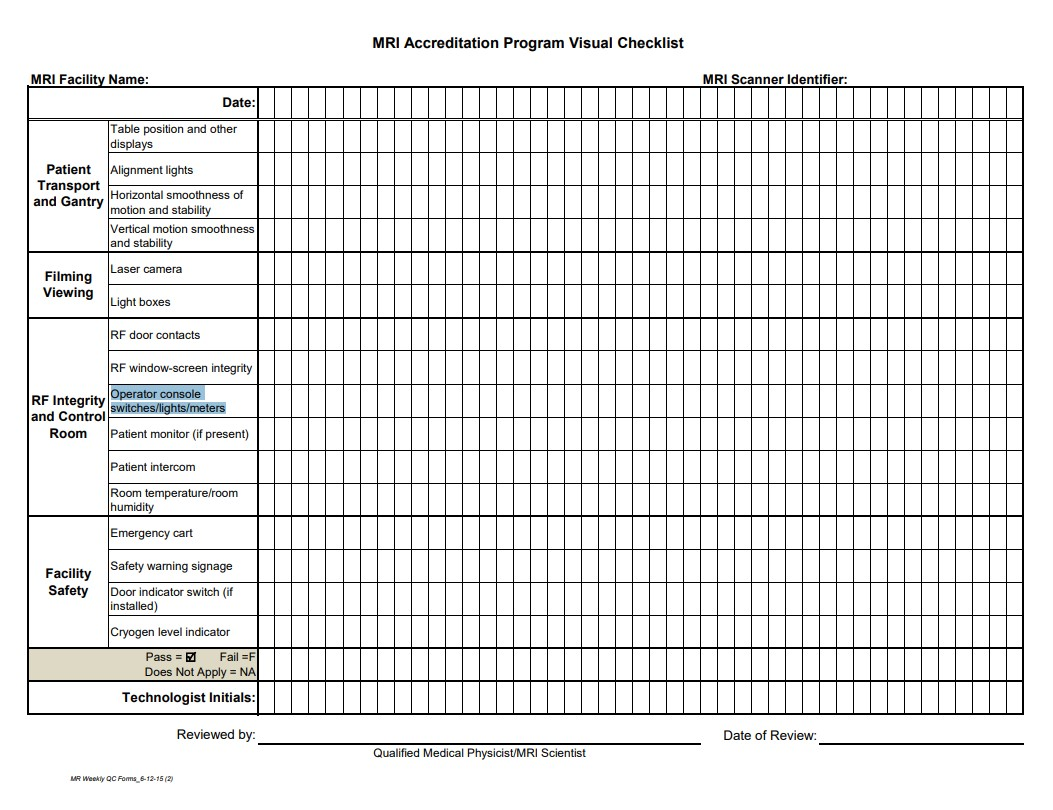
\includegraphics[width=0.8\linewidth]{vc.jpg}
    \caption{\small{Visual checklist for MRI}}
    \label{fig:Visual checklist for MRI}
\end{figure}

If any of this fails, it should be repaired or replaced as soon as possible even before carrying out other quality assurance protocols. 

\newcommand{\mysubscript}[1]{\raisebox{-0.34ex}{\scriptsize#1}}

\subsection{Setup and Table Position Accuracy Test}
Setup and Table Position Accuracy is a method used to determine that the MRI machine performs patient setup, data entry and prescan tasks properly. And this should be done once a week. For this QA test a MRI phantom is used. Method of using the phantom is shown in the following figure. If the positioning laser is calibrated properly and the table is positioned properly this test is passed.  
\begin{figure}[h!]
    \centering
    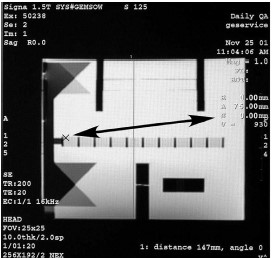
\includegraphics[width=0.3\linewidth]{ph1.jpg}
    \caption{\small{An example taken from a scanner where a square ROI has been placed with its center on the anterior/superior edge of the grid}}
    \label{fig:An example taken from a scanner where a square ROI has been placed
with its center on the anterior/superior edge of the grid}
\end{figure}

\begin{figure}[h!]
    \centering
    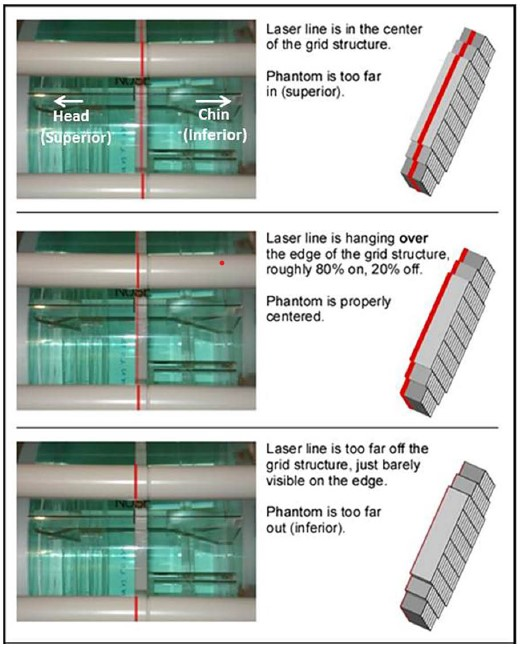
\includegraphics[width=0.7\linewidth]{ph.jpg}
    \caption{\small{Illustration of the use of the central grid structure for alignment of the large phantom}}
    \label{fig:Illustration of the use of the central grid structure for alignment of the large phantom}
\end{figure}


\subsection{Center Frequency Test}
The resonance frequency is the RF frequency that matches with the magnetic field intensity \textit B(Tesla)

\begin{equation*}
    f = \frac{\gamma}{2\pi}\times B
\end{equation*}

MRI system manufacturers provides specific automated protocols for resonance frequency adjustments. Using the phantom at the center of the magnetic field RF frequency us adjusted. Working the system off the frequency reduces the SNR value and the quality of the image. A MRI phantom is used for this test. This test has to be done weekly. If the recorded center frequency value does not match with value established by the qualified medical physicist or MRI scientist, the test should be repeated. If the test proved to be correct by the second test, re correction need to be done for the RF frequency before other QA protocols are executed. 

\subsection{Transmitter Gain or Attenuation Test}
Transmitter Gain or Attenuation Test is protocol followed once a week. If there are any fluctuations in transmitter Gain or Attenuation there are problems associated with the RF chain. This test is done after tuning the resonance frequency and it acquires several signal while varying the transmitter gain. If the changes measured in Transmitter attenuation or gain exceeds the limits MRI system should be subjected to repair. This is very important since transmitter gain is directly related to SNR value. 

\subsection{Geometric Accuracy Measurement Test}
Geometric Accuracy Measurement test is carried out with a MRI accreditation phantom and frequency of the test is once in a week. Objective of this test is to verify that the image taken from the system(outcome) has the similar dimensions with the body part. 
\begin{equation*}
    \textit{GD\%} = \frac{true_dimension-observed_dimension}{true_dimension}\times 100
\end{equation*}

\begin{figure}[h!]
    \centering
    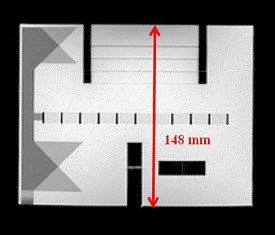
\includegraphics[width=0.5\linewidth]{ph2.jpg}
    \caption{\small{Positioning of length measurement on ACR MR accreditation phantom.}}
    \label{fig:Positioning of length measurement on ACR MR accreditation phantom.}
\end{figure}
If the MRI is not properly calibrated or the faults in the gradient scaling factors which may produce a non homogeneous magnetic field, this test might not pass. If the test is failed it is better find out which of the above problem caused it. 
\subsection{High-Contrast Spatial Resolution Test}
High-contrast Spatial Resolution Test; also known as "Limiting spatial resolution" measures the ability of MRI system to resolve small objects. When the scanner has the ability to resolve small details of a object it has a good spatial resolution. This test is also done by a MRI accreditation phantom. 
\begin{figure}[h!]
    \centering
    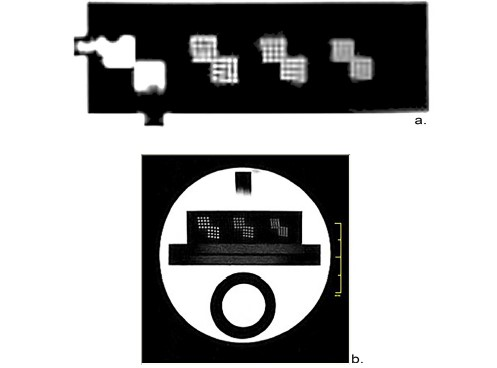
\includegraphics[width=0.7\linewidth]{ph3.jpg}
    \caption{\small{a) Large phantom high-contrast resolution insert from slice 1 of an axial series shows three sets of two arrays of holes. Hole sizes and spacing: from left, 1.1 mm, 1.0 mm, and 0.9 mm. b) Small phantom high-contrast resolution insert from slice 1. Hole sizes and spacing: from left, 0.9 mm, 0.8 mm, and 0.7 mm.}}
    \label{fig:a) Large phantom high-contrast resolution insert from slice 1 of an axial series shows three sets of two arrays of holes. Hole sizes and spacing: from left, 1.1 mm, 1.0 mm, and 0.9 mm. b) Small phantom high-contrast resolution insert from slice 1. Hole sizes and spacing: from left, 0.9 mm, 0.8 mm, and 0.7 mm.}
\end{figure}

\subsection{Low-Contrast Detectability Test}
The low-contrast detectability (LCD) test measures the extent to which objects of low contrast are discernible in the images. For this purpose the MRI accreditation phantom is used which contains contrast objects of varying size and contrast. The detection of a low-contrast object is primarily determined by the contrast-to-noise ratio achieved in the image, and may be reduced due to the presence of artifacts such as ghosting. It should be carried out weekly. 

Following figure shows the difference of the Low-contrast detectability of two different MRI machines of 1.5T scanner (left) and 0.3T scanner (right).
\begin{figure}[h!]
    \centering
    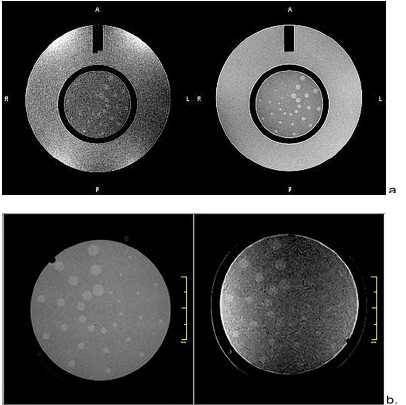
\includegraphics[width=0.6\linewidth]{ph4.jpg}
    \caption{\small{Phantom images of low-contrast detectability (LCD) inserts.}}
    \label{fig:Phantom images of low-contrast detectability (LCD) inserts.}
\end{figure}

\begin{enumerate}[a)]
    \item Large phantom LCD insert images. Slice 11 (5.1\% contrast) acquired on two different scanners, each with proper slice positioning. The left image is from a 1.5T scanner where all 10 spokes (each spoke consisting of three test objects) are visible. Right image is from slice 11 of a 0.3T scanner where only seven complete spokes are visible. The qualified medical physicist or MRI scientist should designate the specific  MRI phantom image slice that is most appropriate to assess for weekly
    \item Small phantom LCD insert images. The left image is slice 7 (5.1\% contrast) from a 1T scanner, where all 10 spokes are visible. The right image is also slice 7, but from a 0.3T scanner, where 7 spokes are visible. One or two objects in the eighth spoke are seen, but the outermost object is no more apparent than background noise, so the eighth spoke is not counted, nor are any spokes beyond the eighth spoke.
\end{enumerate}
\subsection{Artifact Evaluation Test}
Artifact Evaluation test is a artifact analysis procedure. This could be a early measurement of declining system performance. This test is done in every week with the use of a phantom. 
Following scenarios should be true if the system performs normal during the test.
\begin{enumerate}[i.]
    \item Phantom appears circular, not distorted
    \item No ghost images appears over the phantom or in the background
    \item There are no bright/dark spots or streaks
    \item There no unusual new feature in the image
\end{enumerate}

\subsection{Film Printer Quality Control Test}
This test assures that the films produced are artefact free and and consistent with gray levels. This test should be done as necessary when a change happens in the film system. Ex: change of chemicals/film type. There is no specific time for this test. Equipments used for this tests are,
\begin{enumerate}[i.]
    \item Densitometer
    \item Film printer QC chart
\end{enumerate}
\begin{figure}[h!]
    \centering
    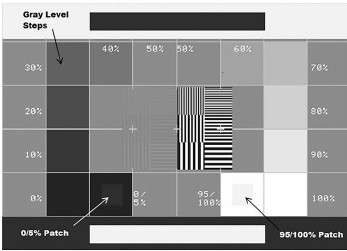
\includegraphics[width=0.5\linewidth]{ph5.jpg}
    \caption{\small{The central portion of the test pattern}}
    \label{fig:The central portion of the SMPTE test pattern}
\end{figure}
If the gray levels on the film matches with the gray levels on the display the Film system qualified to proceed from this test. 

\subsection{Magnetic Field Homogeneity Test}
Homogeneity of the main magnetic field in the designated volume is one of the most important condition in MRI systems. Magnetic field inhomogeneity is usually specified in parts per million (ppm) of the magnetic field strength over a spherical volume. Inhomogeneities  contributes to difficulty in obtaining fat suppression and geometrical distortions of images. 

When comparing with other Quality assurance methods this procedure might be the hardest one. This test must be carried out annually. There are 4 methods for this test. They are,
\begin{enumerate}[i.]
    \item Spectral peak method
    \item Bandwidth-difference method
    \item Phase-map method
    \item Phase-difference method
\end{enumerate}
\begin{figure}[h!]
    \centering
    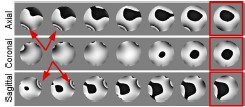
\includegraphics[width=0.5\linewidth]{ph6.jpg}
    \caption{\small{Boxes in the right appears to be completely normal while, inhomogeneities are appeared to be in the left by the arrows which was caused due to a bobby pin under the magnet bore}}
    \label{fig:The central portion of the SMPTE test pattern}
\end{figure}

\subsection{Slice-Position Accuracy Test}
Slice Position Accuracy test assures the accuracy of the axial slices which are positioned at specific locations. It helps to determine whether the actual locations of acquired slices differ from their position in the image. Following procedure has to done to each image in this test.
\begin{enumerate}[i.]
    \item Display the slice magnified on the monitor by a factor of two to four.
    \item Adjust the display window so that the ends of the vertical bars are not fuzzy using a narrow window width.
    \item Use the viewer’s length measurement tool to determine the difference in length between the left and right bars.
    \item Record the measured data in the annual system performance evaluation report.
\end{enumerate}


\subsection{Slice-Thickness Accuracy Test}
Slice-Thickness Accuracy test is executed annually to assess the accuracy of a specified slice thickness. The measured slice thickness is compared with the prescribed slice thickness. Low slice thickness accuracy might not suggest that the slices are too thin or thick but also due to the image contrast and SNR value. 

Slice thickness value is calculated using the following formula.
\begin{equation*}
Slice_thickness = 0.2 \times \frac{top\times bottom}{top + bottom}
\end{equation*}
where “top” and “bottom” are the measured lengths of the top and bottom
signal ramps. 
\subsection{Radio-frequency Coils Checks }
Radio-frequency Coils checks ensures that the perfect radio-frequency is generated. Otherwise noise in the image will be high and SNR will be low. MRI vendor supplies the tools to check the radio-frequency coils. 


\subsubsection{SNR}
There are two methods to measure the SNR,
\begin{enumerate}
    \item Single-Image SNR Method\newline
    Select an image of the phantom that is depicting its center along the central axis. Then create a mean signal region of interest that covers at least 0.75 of the cross sectional area of the phantom. Observe the mean signal - the average value of all the pixels in the defined region. Place a measurement ROI of as large as possible in a position in the background area outside the phantom volume in the frequency-encoding direction. And obtain the background noise and signal measurements. 
    \begin{figure}[h!]
        \centering
        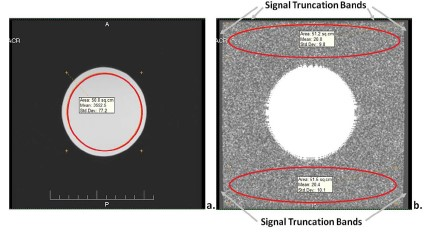
\includegraphics[width=0.5\linewidth]{ph7.jpg}
        \caption{\small{Single Image SNR Method}}
        \label{fig:Single Image SNR Method}
    \end{figure}
    \begin{equation*}
        SNR = \frac{Mean\_Signal\_in\_Phantom}{\sigma}
    \end{equation*}
   ;where $\sigma$ = standard deviation in the air ROI   
    
    \item Two-Image SNR Method \newline
    In this method first step is to acquire two identical images of a uniform homogeneous phantom at the same time. Then in the one of the image a mean signal region of interest is defined(more than 75\% of the whole image). Then record the mean signal which is the average of the all the pixels in the mean signal ROI. Then create the difference by subtracting each other. The difference image is used to create two more similar regions of interests and define the mean signal and determine the standard deviation.
    \begin{equation*}
        SNR = \sqrt{2} \times \frac{Mean\_Signal}{\sigma}
    \end{equation*}
    \begin{figure}[h!]
        \centering
        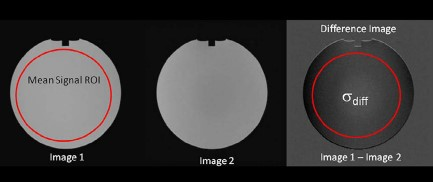
\includegraphics[width=0.5\linewidth]{ph8.jpg}
        \caption{\small{Two-Image SNR Method}}
        \label{fig:Two Image SNR Method}
    \end{figure}
\end{enumerate}
\subsubsection{Percent Image Uniformity (PUI)}
This is test carried out annually to measure the uniformity of the image using a uniform cylindrical phantom. Here windowing is done in two ways. First time only the brightest points are seen. Second time only the darkest points are seen as shown in the following figure. From the both of the images define a region of interest which includes all the brightest and darkest spots.  And measure mean signal values in each pixel. PIU is calculated from the following equation. 
\begin{equation*}
    PIU = 100 \times (1 - \frac{Max\_ROI - Min\_ROI}{Max\_ROI -=+ Min\_ROI})
\end{equation*}
\begin{figure}[h!]
    \centering
    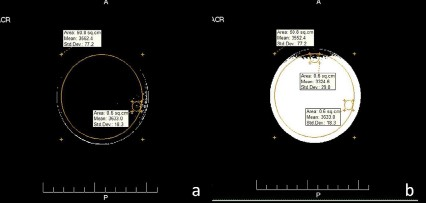
\includegraphics[width=0.5\linewidth]{ph9.jpg}
    \caption{\small{PIU Test}}
    \label{fig:PIU Test}
\end{figure}

\subsubsection{Percent Signal Ghosting (PSG)}
Percent Signal Ghosting - PSG is a measurement of the phenomenon known as "Ghosting" which occurs due to movements of the subject. Even the blood flow causes the ghosting phenomenon. It is measured by following procedure. 

First establish measurements ROIs in the four positions as shown in following figure. Then record each measured signal values. And calculate PSG value using following equation. 

\begin{equation*}
    PSG = 100 \times |\frac{(Left+Right)-(Top+Bottom)}{2 \times MEan\_signal}|
\end{equation*}
\begin{figure}[h!]
    \centering
    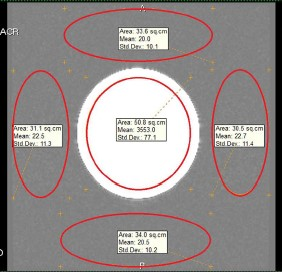
\includegraphics[width=0.5\linewidth]{ph10.jpg}
    \caption{\small{Placement of ROIs inside and outside the phantom to determine percent signal ghosting}}
    \label{fig:PSG test}
\end{figure}

% \subsection{Soft-copy (Monitor) Quality COntrol Test}
% \subsection{MR Safety Program Assessment Test}





% \subsection{Water CT Number}

% CT number is a measurement of the linear attenuation coefficient of a material. CT number is denoted in Hounsfield Unit (HU). The Hounsfield Unit is based on the ratio of the linear attenuation coefficients of water and the material of interests. It is given by,

% \begin{equation*}
%     HU = \frac{\mu - \mu\mysubscript{Water}}{\mu\mysubscript{Water}-\mu\mysubscript{Air}}
% \end{equation*}
% \begin{equation*}
%     \mu = linear\hspace{0.3 cm} attenuation\hspace{0.3 cm} coefficient\hspace{0.3 cm} of \hspace{0.3 cm}the \hspace{0.3 cm}material
% \end{equation*}
% \begin{equation*}
%     \mu\mysubscript{Water} = linear\hspace{0.3 cm} attenuation\hspace{0.3 cm} coefficient\hspace{0.3 cm} of\hspace{0.3 cm} distilled \hspace{0.3 cm}water\hspace{0.3 cm} at\hspace{0.3 cm} STP   
% \end{equation*}
% \begin{equation*}
%     \mu\mysubscript{Air} = linear \hspace{0.3 cm}attenuation \hspace{0.3 cm}coefficient\hspace{0.3 cm} of \hspace{0.3 cm}air \hspace{0.3 cm}at\hspace{0.3 cm} STP
% \end{equation*}

% To ensure the constancy of the CT imaging system, it is required to check whether the images obtained by the CT system remains invariant over a period. This is done by imaging a standard object called a phantom and comparing the outcome with the expected outcome. In CT, this is carried out as the measurement of water CT number. A water phantom is usually provided by the equipment manufacturer for this purpose. A CT image is obtained using this phantom as the imaged object. Sample CT slices should be obtained from the middle part of the phantom and the initial or trailing parts. This procedure should be done for both axial and helical canning modes. The settings used for imaging should be the standard CT parameters set for usual clinical imaging parameters.

% Two measurements are obtained for this phantom. The mean Hounsfield number of this phantom and the standard deviation. While the mean should ideally be Zero, the variance should satisfy the boundaries set by the manufacturer. However, the limits can be set by the clinical engineer based on the conditions under which the image is obtained, in the case that custom setting were used for the imaging other than the standard prescribed by the manufacturer. Typically the mean should satisfy the following limits for the CT system to be evaluated as normally functioning.

% \begin{equation*}
%     mean = 0 \pm 3  \hspace{0.3 cm} HU
% \end{equation*}

% However, irrespective of the settings used the absolute maximum deviation of the mean that is tolerable is ±5 \textit{HU}. The Standard deviation of the Hounsfield Number corresponds to the noisiness of the imaging system. Therefore this corresponds to the radiation dosage used and thus the limits should be decided by the clinical engineer performing the test based on the scan technique. If he chooses to use the limits provided by the manufacturer, he should obtain the phantom image according to the manufacturer’s recommended scan techniques (reconstructed image thickness and filters used for reconstruction). Instead of water phantoms various other standard CT phantoms can be used to evaluate the constancy of the imaging system. However, the limits of acceptability should be obtained from the standards for the phantom used. Usually if mean and variance values fall outside the recommended limits for 3 consecutive tests performed within a week, the constancy of the system is considered to be lost. If the measures indicate that there is some loss of constancy, further tests must be done to isolate the cause of the problem and repairs or replacements should be done.

% \subsection{Review of Clinical Protocols}

% In every imaging modality there are several specified guidelines to obey when using the system. Those are the clinical protocols of the system. But those procedures may differ according to the patient. To keep the procedures constant over a period of time the parameters, settings and conditions used for imaging for each type of patient and image requirements is reviewed and agreed upon. This protocol is strictly followed in order to avoid mistakes and inconsistencies.

% In every imaging system following protocols are used for imaging,
% \begin{itemize}
%     \item Pediatric head CT (1 year old)
%     \item Pediatric abdominal CT (5 years ; 20 kg)
%     \item Adult head CT
%     \item Adult abdomen CT (about 70 kg)
%     \item High-resolution chest CT
%     \item Brain perfusion CT
% \end{itemize}

% There is a set for all the parameters involved in the imaging procedure For each of these CT protocols. Based on the type of image and normally consist of the following special parameters specific for only some protocols must be included as well.

% \begin{enumerate}
%     \item Tube Voltage - kV
%     \item Tube Current - mA
%     \item Rotation time
%     \item Pitch
%     \item Configuration of the detector
%     \item Reconstructed image thickness
%     \item Reconstruction algorithm or kernels
%     \item Breath-hold time
    
% \end{enumerate}

% \textbf{Computed Tomography Dose Index} - \textbf{CTDI} is a measure of the radiation dose that is emitted from the CT source. While this is not a measure of the radiation dose that is received by a patient under scanning, it is considered that \textbf{CTDI} is a better measurement in regulation and quality control of the radiation. The reason for this is the impractical nature of measuring the actual radiation dose received by the patient during scanning. In reviewing protocols it is necessary to make sure that the \textbf{CTDI} values are in accordance with the recommended values. \textbf{CTDI} can be evaluated both before imaging patient using the CT displayed parameters and after image acquisition based on the recorded images.

% \subsection{Rules and Regulations}

% There are rules and regulations for the for radiologists and medical practitioners including medical engineers. Following are few examples for such rules and regualtions,

% \begin{itemize}
%     \item Reconstructed image thickness of standard adult head and abdomen CT should be less than 5 mm.
%     \item Minimum possible rotation time for pediatric abdomen should be chosen
%     \item Maximum value of detector configuration or beam collimation should be used whenever practical, to improve dose efficiency. Here beam collimation is expressed as NT defined by,
%     \begin{equation*}
%         NT = N \times T
%     \end{equation*}
%     With N is the number of X ray channels and T is the thickness of one channel. For example, 4 × 5 mm collimation is up to 30\% more dose efficient than 2 × 5 mm collimation in axial mode with no loss in image quality.
%     \item Lower kV settings should be used for pediatric scans and scans that use oral or intravenous contrast agents
%     \item High-Resolution Chest (HRC) protocol should sharp filters and should be axial images of thin slices about 10-20 mm apart. If helical images are obtained it should be made sure that diagnostic usefulness is ensured.
%     \item Minimum possible dose should be used. The recommended CTDI should never be exceeded for the standard protocols. Radiation dose thresholds should be designed for any custom CT protocol
% \end{itemize}

% \subsection{Table travel accuracy}
% This is a quality assurance method of the x-ray source. This test is use to test the accuracy of the patient table's translational movements. There is a procedure with few steps to conduct this test. If the test fails to prove the accuracy the table need to be repaired. 

% Following are the steps,
% \begin{enumerate}
%     \item Place the special phantom and align the first marker with the axial plane
%     \item Add some weight to the table top to simulate it to an actual persons weight
%     \item Set the table position indication to zero.
%     \item Slide the table to align for the second marker.
%     \item Record the position of the table
%     \item slide the table to the maximum possible extension and return to the first marker
%     \item Record the new position of the table
% \end{enumerate}

% \pagebreak

% \subsection{Dosimetry}
% Dosimetry is the measurement of the radiation dose received by the patient during a CT scan. Prior to performing the scan the scanner  provides an calculated Computed Tomography Dose Index (CTDI).

% By doing this test it can be verified whether the indicated dose is accurate to the real radiation exposure of the patient. This is need to be done twice in a year to maintain the quality. 

% A special phantom with holes is used for this. It is connected to an electrometer that measures the radiation exposure of the chamber along its length. Following figure shows such phantom,
% \begin{figure}[h!]
%   \centering
%   \includegraphics[width=0.45\linewidth]{phantom.jpg}
%   \caption{\small{Phantom toolkit for CT}}
%   \label{fig:Phantom toolkit for CT}
% \end{figure}

% \subsection{Alignment Light Accuracy}
% Alignment lights are used to check the alignment of the patient. If the alignment is wrong the patient might have to once again. And vulnerable organs of the body can be exposed to radiations. Thus, before doing the imaging, patient is aligned using a light source. A CT phantom with a marker that is opaque to X-rays is placed on the CT table using the alignment light as a guide and the table position is set to zero. A series of images are acquired around this position with about 0.5 mm gap between each slice. Once the obtained images are obtained, the most clearly visible image slices location is found. This distance corresponds to the axial misalignment of the alignment light. If the misalignment is more than 2mm corrective action should be done to restore it to below that limit. 

% \subsection{Radiation Beam Width}
% Radiation beam width test is used to measure the width of the radiation beam. The optimal value indicated in the scanner differs with the actual width of the X-ray beam. But this gap should be in a safe range otherwise patient is in danger. Therefore this method is used to protect the patient while getting the best results from the imaging

% \subsection{Artifact Evaluation}
% Artefacts affects the readability of  the image because they would mimic features that are not present in the imaged body. Therefore, artefact evaluation tests must be carried out daily to identify the occurrence of artefacts.

% \begin{figure}[h!]
%   \centering
%   \includegraphics[width=0.75\linewidth]{ar.jpg}
%   \caption{\small{Identified artifacts in a CT image}}
%   \label{fig:Identified artifacts in a CT image}
% \end{figure}

% %\subsection{Image Thickness}
% \subsection{Spatial Resolution}
% This test is performed to verify that the spatial resolution of the CT imaging is sufficient for clinical diagnosis. This test must be done annually or whenever a significant change is done to the system. The following procedure is carried out to evaluate the spatial resolution. 
% \begin{enumerate}
%     \item The phantom is correctly aligned to the resolution measurement area
%     \item Set mA parameters manually to suit the image
%     \item Obtain the following scan protocols
%     \begin{enumerate}
%         \item Adult abdomen
%         \item High-resolution chest
%     \end{enumerate}
    
%     \item Select the image where the contrast indication area is closest to the center
%     \item Determine the highest resolution that is visible
% (The resolution at which any further increase makes the lines appear as a continuous block)
%     \item 6. Select suitable reconstruction algorithm (Sharp reconstruction for chest imaging)
% \end{enumerate}

% \begin{figure}[h!]
%   \centering
%   \includegraphics[width=0.55\linewidth]{sr.png}
%   \caption{\small{High contrast spatial resolution for seven volumetric imaging systems}}
%   \label{fig:High contrast spatial resolution for seven volumetric imaging systems}
% \end{figure}

% Necessary actions should be taken after checking those values and comparing with the recommended values. 

% \subsection{CT number accuracy and Uniformity}
% The CT number measured in \textit{Hounsfield} Units is the primary measurement of CT images. Therefore it is required to make sure that the CT number is accurate, Different phantoms with embedded materials with known CT number (Different linear attenuation) are used for this purpose. The test should be performed for several imaging protocols and different \textit{kV} settings annually or after major modifications to the system.

% \begin{figure}[h!]
%   \centering
%   \includegraphics[width=0.75\linewidth]{CTN.png}
%   \caption{\small{Parameter variation with time}}
%   \label{fig:Parameter variation with time}
% \end{figure}
% %\subsection{Low Contrast Performance}

\pagebreak
\section{Recent advancements in \thetitle}
MRI systems are highly technological devices. As the science and technology develops MRI systems get more chance to develop their performances. Early MRI systems were consisted of permanent magnets with low magnetic power. After then electromagnets were used. But after the discovery of superconductors it was a huge step for the MRI systems. Totally new technology was developed. From the beginning in 1970s, MRI systems were developed in big steps.So were the quality assurance technologies. As the technology develops, it needs more accurate quality assurance methods. 

Phantoms are widely used in MRI quality assurance. Normally water based phantoms are used for MRI quality assurance. But due to inconvenience of using water phantoms, now scientists are researching for a substance that can replace water phantoms. BEAMSCAN is a such developed phantom and dosimeter system that is of higher accuracy even if it measures the parameter in less than half the conventional time. The phantom can be controlled and monitored through remotely connected computers using wireless communication.

\begin{figure}[h!]
  \centering
  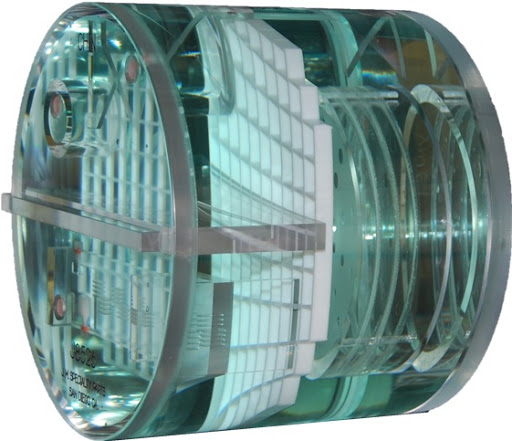
\includegraphics[width=0.3\linewidth]{p.jpg}
  \caption{\small{Phantom toolkit for MRI}}
  \label{fig:Phantom toolkit for MRI}
\end{figure}
\begin{figure}[h!]
  \centering
  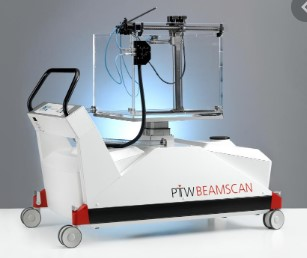
\includegraphics[width=0.3\linewidth]{beam.jpg}
  \caption{\small{BEAMSCAN}}
  \label{fig:Phantom Beamscan toolkit for MRI}
\end{figure}

\pagebreak
\section{Reference}
\begin{enumerate}
    \item Magnetic resonance imaging (MRI) quality control manual: 2015. Reston, VA: American College of Radiology, 2015.
    \item Brown, M. A., \& Semelka, R. C. (2011). MRI: Basic Principles and Applications (2nd ed.). Chicester: John Wiley \& Sons, Inc.
    \item A. R. Webb, Introduction to biomedical imaging. Hoboken, N. J.: John Wiley \& Sons, 2006.
    \item https://www.acraccreditation.org/-/media/ACRAccreditation/Documents/MRI/MR-Visual-Checklist-11614.pdf?la=en
    \item “Magnetic Resonance Imaging - American College of Radiology.” [Online]. Available: https://studyres.com/doc/1590501/magnetic-resonance-. [Accessed: 10-May-2020].
    
    
\end{enumerate}
\pagebreak
\textbf{\Large{Appendix}}
\begin{appendix}
  \listoffigures
  %\listoftables
\end{appendix}

\end{document}

